\documentclass[11pt,a4paper,twoside]{article}

% You should not change the line above.
% Nor change any of the formating.

% At a minimum, you need to edit the preamble file for your name and project
% title. There are a lot of latex commands there you might find useful.
\usepackage[a4paper]{geometry}
\usepackage{amsfonts}
\usepackage{amsthm}
\usepackage{amsmath}
\usepackage{parskip}
\usepackage{mathrsfs}
\usepackage{graphicx}
\usepackage{amssymb}
\usepackage{gensymb}
\usepackage{xtab}
\usepackage{tikz}
% You need to set the next two items. 
% If you title is long, you may need to adjust the spacing in titlepage.tex
\newcommand{\TheAuthor}{Lyllian Chanerley}
\newcommand{\TheTitle}{The Interfacial Dynamics of Bursting Bubbles}

% uncomment exacly one of these
%\newcommand{\TheModule}{\bf MA4K8 Scholarly Report}
\newcommand{\TheModule}{\bf MA4K9 Dissertation}


% Leave the following two as is
\newcommand{\TheUni}{The University of Warwick}
\newcommand{\TheDept}{Mathematics Institute}

% Set the correct submission year, e.g. replace 2000 with 2017
\newcommand{\TheSubDate}{\monthyear \formatdate{5}{4}{2025}}

% The are a lot of things you might find useful and want to uncomment. 
% Most things you will want to uncomment or change will be near the top.

% standard maths symbols (you probably want to uncomment all of these)
% \newcommand{\Z}{\ensuremath{\mathbb{Z}}}% integers
% \newcommand{\N}{\ensuremath{\mathbb{N}}}% natural numbers
% \newcommand{\R}{\ensuremath{\mathbb{R}}}% real numbers
% \newcommand{\C}{\ensuremath{\mathbb{C}}}% complex numbers

% Others 
\newcommand{\st}{\ensuremath{:}}% such that
\newcommand{\Tau}{\ensuremath{\mathcal{T}}}
\newcommand{\Nat}{\mathbb{N}}

\newenvironment{rcases}   
{\left.\begin{aligned}}  
 {\end{aligned}\right\rbrace}

\usepackage[numbers]{natbib}% round braces, sort multiple citations
\usepackage{hyperref}% creates hypertext links in pdf files (natbib compatible)
\usepackage{setspace}
\usepackage{fancyhdr}
\usepackage{mathrsfs}
\usepackage{textcomp}
\usepackage{color}
\usepackage{graphicx}
\usepackage{framed}
 \usepackage{algorithmic}% format pseudocode
\usepackage[vlined,boxed,commentsnumbered,algochapter]{algorithm2e}
 \usepackage[chapter]{algorithm}% float wrapper for algorithms
\usepackage{amsmath}% American Mathematical Society macros - essential!
\usepackage{amssymb}% contains amsfonts
\usepackage{amsthm}% allows more flexibility with theorems
\usepackage[nodayofweek]{datetime} % change the format of printed dates (no american style!) 
\usepackage{ifdraft}% perform operations conditional on the draft option

% \usepackage{mathptmx}
% \usepackage{mathpazo}
%\usepackage{amscd}
% \usepackage{xy}
% \usepackage{diagxy}
%\usepackage{diagrams}

%\usepackage{marginnote}
%\usepackage{rotating}
%\usepackage{multirow}
% \usepackage{polski}
% \usepackage[T1]{fontenc}
% \usepackage{tikzpicture}
% \usetikzlibrary{matrix,arrows}

% \usepackage[inline]{showlabels}
%\usepackage{booktabs}

% Date format

% Use the datetime package
\newdateformat{monthyear}{\monthname[\THEMONTH], \THEYEAR}% new date format

% New commands, operators and symbols

% Operators
%\DeclareMathOperator{\Sym}{Sym}% symmetric group
%\DeclareMathOperator{\Alt}{Alt}% alternating group
%\DeclareMathOperator{\Id}{Id}
%\DeclareMathOperator{\Hom}{Hom}
%\DeclareMathOperator{\Grp}{Grp}
%\DeclareMathOperator{\supp}{supp}
%\DeclareMathOperator{\fix}{fix}
%\DeclareMathOperator{\dep}{dep}
%\DeclareMathOperator{\lcm}{lcm}
%\DeclareMathOperator{\Aut}{Aut}
%\DeclareMathOperator{\Inn}{Inn}
%\DeclareMathOperator{\Out}{Out}
% \DeclareMathOperator{\dim}{dim}
%\DeclareMathOperator{\Syl}{Syl}
%\DeclareMathOperator{\Hall}{Hall}
%\DeclareMathOperator{\pCore}{pCore}
%\DeclareMathOperator{\Char}{char}
%\DeclareMathOperator{\Image}{Im}
%\DeclareMathOperator{\Ker}{Ker}
%\DeclareMathOperator{\Hcf}{hcf}
%\DeclareMathOperator{\GL}{GL}
%\DeclareMathOperator{\Pc}{Pc}
%\DeclareMathOperator{\Stab}{Stab}
%\DeclareMathOperator{\Orbit}{Orbit}


% Hyphenation fixes
%\newcommand{\letdash}[1]{$#1$\nobreakdash-\hspace{0pt}}% for n-element, k-transitive etc
%\newcommand{\numdash}{\nobreakdash--}

% Sequences
%\newcommand{\seqfin}[3]{\ensuremath{#1_{#2}, \dotsc , #1_{#3}}}
%\newcommand{\seqinf}[3]{\ensuremath{#1_{#2}, #1_{#3}, \dotsc}}

% New environments

% Dedication
%\newenvironment{dedication}
%{\clearpage \thispagestyle{empty} \vspace*{\stretch{1}} \begin{center} \em}
%{\end{center} \vspace*{\stretch{3}} \clearpage}


% Page Layout

% Dimensions
% Use the geometry package to set this up
\geometry{includehead,includefoot,left=3cm,right=3cm,top=2cm,bottom=2cm}% head and foot are included in total body so that nothing is printed out of the boundaries of the set margins

% Header and footer
% Use the fancydr package
%\ifdraft{%
%\fancypagestyle{plain}{% redefine plain pagestyle for draft
%\renewcommand{\headrulewidth}{0pt}% no head rule in draft mode
%\fancyhf{}% clear headers and footers
%\fancyhead[C]{\ifdraft{DRAFT}{}}% print DRAFT across top if the draft option is set
%\fancyfoot[C]{\thepage}% usual page numbering
%

%\pagestyle{fancy}
%\renewcommand{\chaptermark}[1]{\markboth{\thechapter.\ #1}{}}% compact with no capitalisation
%\renewcommand{\sectionmark}[1]{\markright{\thesection.\ #1}}% compact with no capitalisation
%\ifdraft{\renewcommand{\headrulewidth}{0pt}}{}% no head rule in draft mode
%\setlength{\headheight}{15pt}
%\fancyhf{}% clear all header and footer fields
% one-sided printing, so no E,O distinction need be made
%\fancyhead[C]{\ifdraft{DRAFT}{}}% print DRAFT across top if the draft option is set
%\fancyhead[R]{\thepage}% page in top right
%\fancyhead[L]{\ifdraft{}{\leftmark}}% chapter number and title in top left

% Theorems
%
%\newtheorem{prop}{Proposition}[chapter]
%\newtheorem{lemma}[prop]{Lemma}
%\newtheorem{conjecture}[prop]{Conjecture}
%\newtheorem{theorem}[prop]{Theorem}
%\newtheorem{hyp}[prop]{Hypothesis}
%\newtheorem{cor}[prop]{Corollary}
%\newtheorem{claim}[prop]{Claim}
%\newtheorem{remark}[prop]{Remark}
%\newtheorem{notation}[prop]{Notation}
%\newtheorem{defn}[prop]{Definition}


% Numbering
%\numberwithin{equation}{chapter}% standard style numbering, nothing special here


% Algorithms

% Use the algorithms package.
% \renewcommand{\algorithmicrequire}{\textbf{Input:}}
% \renewcommand{\algorithmicensure}{\textbf{Output:}}
% \renewcommand{\algorithmiccomment}[1]{/* #1 */}
%\RestyleAlgo{boxruled}
%\SetAlgoInsideSkip{medskip}
%\setlength{\algomargin}{2em}
%\setlength{\interspacetitleboxruled}{0.7em}
%\setlength{\interspacetitleruled}{0.7em}
%\LinesNumbered
%\SetAlCapNameSty{sc}
%\SetFuncSty{sc}

%\newenvironment{spacedalgorithm}{\begin{algorithm}\onehalfspacing}{\end{algorithm}}
% \newenvironment{onehalfverbatim}{\onehalfspacing\begin{verbatim}}{\end{verbatim}}

%\reversemarginpar
%\newcounter{nootje}
%\setcounter{nootje}{1}
%\renewcommand\check[1]{[*\thenootje]\marginnote{\tiny\begin{minipage}{40mm}\begin{flushright}\thenootje
%: #1\end{flushright}\end{minipage}}\addtocounter{nootje}{1}}


% Document details



\begin{document}

\pagenumbering{roman}
\begin{titlepage}
\begin{center}

\includegraphics[width=5cm]{Warwick_Crest} 
% this graphic file should live in the working directory
% the size of the following arguments to vspace were determined by 
% trial and error, and produce suitable output for the A4 pagesize.

\vspace*{20pt}
\begin{spacing}{2}
\begin{center}
{\Large \bf \TheTitle} % declared in preamble.tex

\vspace*{14pt}

by

{\Large \bf \TheAuthor} % declared in preamble.tex

\vspace*{16pt}

{\large \bf \TheModule} % declared in preamble.tex


Submitted to \TheUni % declared in preamble.tex

\vspace*{36pt}
{\Large \bf \TheDept} % declared in preamble.tex

\TheSubDate % declared in preamble.tex

\vspace*{36pt}

\includegraphics[width=5cm]{warwick_logo} 
% this graphic file should live in the working directory

\end{center}
\end{spacing}
\end{center}
\end{titlepage}

\setcounter{page}{2}
%\renewcommand{\contentsname}{Table of contents}
\tableofcontents
\cleardoublepage
\onehalfspacing
\pagenumbering{arabic}
\onehalfspacing
\raggedbottom

% Now starts the main part of the report. 
% Each section/chapter is in a separate file. Two examples are include.
% 
% This part (between TOC and Bibliograpy) must obey:
% for MA4K8 must not exceed 30 pages.
% for MA4K9 the target is approx 30 pages and must not exceed 40 pages.

\section{Introduction}

Bubbles within liquids are incredibly common, occurring in both a wide spectrum of natural and industrial processes \cite{veron2015ocean}. These occurrences can range from water and carbon-dioxide bubbles in magma providing driving forces for an eruption \cite{Volcano} to carbon-dioxide bubbles in champagne enhancing the evaporation of volatile organic compounds dispersed in the liquid phase \cite{WINE}. When a bubble rises to the surface of a liquid, it may burst, scattering many droplets. These droplets are an important process of transport exchange across the liquid gas interface, they are considered the main source of sea spray aerosols \cite{veron2015ocean} and impact air pollution \cite{murphy2016depth} as well as the transmission of infectious diseases \cite{ji2022water,bourouiba2021fluid}. Bubbles formed due to the breaking of waves contribute to the transfer of heat, mass and other contaminants between the oceans and the atmosphere \cite{coantic1980mass}. The formation of ocean spray by bursting bubbles in coastal areas during red tides of harmful algae can bring pathogens into the atmosphere as aerosols causing heath issues \cite{walls2014moving}. The efficiency of this transfer is governed by the initial size and speed of the ejected drops. \cite{coantic1980mass,andreas1995spray}

\begin{figure}[H]
    \centering
    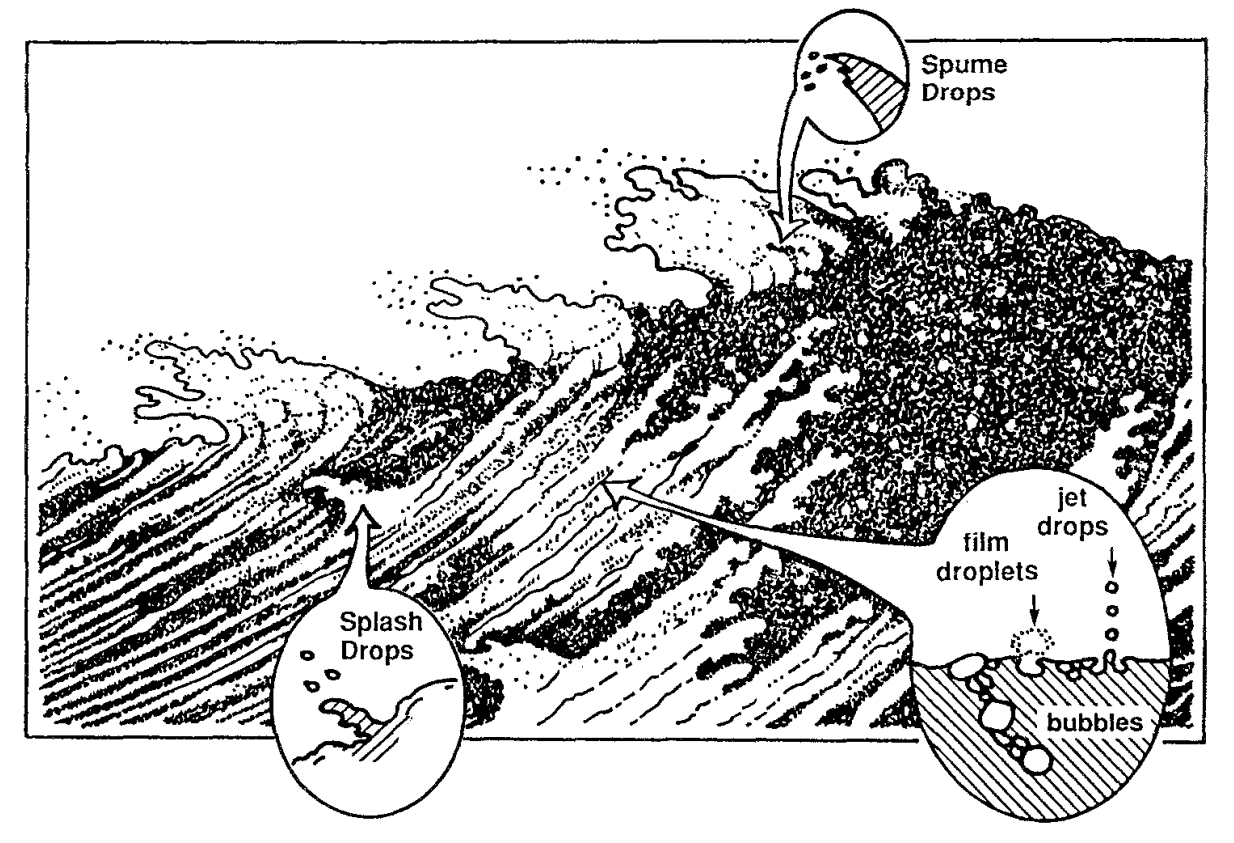
\includegraphics[width=0.8\linewidth]{WriteUp/images/Andreas pic.png}
    \caption{Origin of the various kinds of sea spray droplet. This report focuses on Jet drops Adapted from figure 1 on page 5 of Andreas \textit{et al.} \cite{andreas1995spray} }
    \label{fig:0}
\end{figure}

There are two phenomena that occur when a bubble bursts that produce aerosols, the first being when the thin film separating the bubble from the atmosphere is ruptured. The atomisation of the film can produce several hundred droplets of around a micrometer in diameter. Due to the length scales of the rupture being order O($100$)nm \cite{boulton1993gas}, we are unable to describe this problem with continuum mechanics. In fact, van der Waals forces or electrostatic repulsion must be considered, both of which are long-range intermolecular forces \cite{boulton1993gas}. 

After the film rupture, the remaining cavity collapses causing a jet to form. This jet eventually breaches into one or more droplets. The key difference between these droplets and the droplets formed when the film ruptures is that they are much larger, order O($100 \mu$m) for a typical bubble with a diameter of a millimeter. They are also ejected vertically with a typical ejection velecity of order O($1$ms$^{-1}$).
\begin{figure}[H]
    \centering
    
\includegraphics[width=0.75\linewidth]{WriteUp/images/droplet release 3D.png}
    \caption{An image of jet formation due to a burst bubble.}
    \label{fig:1}
\end{figure}

Since the pioneering study of bursting bubbles by Woodcock \textit{et al.} \cite{woodcock1953giant}, numerous studies have been made documenting jet drop properties. The first comprehensive study using numerical simulations based on a free-surface formulation of the Navier-Stokes equations was done in 2002 by Duchemin \textit{et al.} \cite{duchemin2002jet
}.

In this paper they used a volume-of-fluid (VOF) type method to investigate quantities such as the jet velocity, maximum pressure on the axis of symmetry and radius of the first ejected drop. They compared their numerical data with experimental data published by MacIntyre \cite{macintyre1972flow} and found the overall agreement satisfactory. The method was able to resolve small capillary wave and still accurately predict large scale features of the dynamics, the pressure and final droplet radius.

Another aim of this paper was to investigate bubble entrapment. This is when a new bubble is formed underneath the collapsing cavity of the old bubble. Two entrapment regions were found, the first for $576<R/R_v<2016$ and the second between $57\:600<R/R_v<288\:000$ where $R$ is the radius of the bubble and $R_v=\rho\nu^2/\gamma$ is the viscous-capillary length with $\rho$, $\nu$ and $\gamma$ being liquid density, kinematic viscosity and surface tension respectively. Other regions of entrapment at higher values of $R/R_v$ was speculated but was said to be difficult to observe numerically.

Duchemin \textit{et al.} also showed that the jets are produced by the self-similar collapse of a cavity created by capillary waves. When a bubble cavity is collapsing, small waves form on the cavity interface moving towards the centre of the bubble. due to the symmetrical nature of the phenomenon these waves focus at the centre of the bubble causing a jet to form. These dynamics can be described by a self-similar dynamic based on the balance of inertial and capillary forces \cite{brenner2000jets} and leads to a singularity where the velocity diverges although in reality it is regularised by viscous and capillary effects. Viscosity was shown to play a critical role in the formation of this singularity. Counter-intuitively, the fastest jets are not obtained for a vanishing viscosity, rather they occur in a small range of optimal viscosity. For a Laplace number $\text{La}=\gamma R\rho/\mu^2$ of around $1000$ where $\mu$ is dynamic viscosity, approaches a finite-time singularity for both pressure and velocity. \cite{brenner2000jets} Earlier attempts of numerical simulation used boundary integral methods for inviscid fluids and therefore missed this phenomenon \cite{oguz1993dynamics}.

However, the paper by Duchemin \textit{et al.} was not entirely comprehensive. Many aspects of busting bubbles were not considers, in particular gravity. This lead to a simplified initial condition of a spherical bubble lying just beneath the surface. A hole was then put into the bubble and the sharp edges left over were smoothed to try and prevent numerical singularities. In addition, due to the limited availability fo experimental data at the time, comparisons between the numerical simulations and experimental data was limited and qualitative.

Deike \textit{et al.} tried to rectify these shortcomings in an article where they aimed to verify experimental and numerical results were indeed quantitatively consistent and obtain a complete quantitative description of how the jet velocity depends on both viscosity and gravity and attempt to separate these two effects \cite{deike2018dynamics}. The authors showed that due to the transient nature of the jet formation process, trying to define the jet velocity is incredibly difficult. as a result, throughout the literature there were numerous definitions leading to conflicting reported velocities. They defined the jet velocity as the stationary velocity observed before drop ejection which they found was consistent with most of the experimental measurements \cite{spiel1995births}. They discussed scaling laws involving the Weber number $\text{We}=\rho v^2R/\gamma$ where $v$ is the velocity of the jet, the capillary number $\text{Ca}=\mu v/\gamma$, the Laplace number and the Bond number. They found $\text{We} \propto \text{Bo}^{\beta}$ and $\text{Ca} \propto \text{Bo}^{\beta}$ where $\beta$ depends on the Bond and Laplace numbers. As gravity was now being considered, a more complicated initial condition was used and through direct numerical simulation they were able to separate the roll of gravity (through the Bond number) and viscosity (through the Laplace number). A universal formula was presented linking the jet capillary number to the Bond and Laplace number and found optimal Laplace numbers depending on the Bond number and that the highest velocity is reached for vanishing Bond numbers. When calculating results with $\text{Bo}=0$ they acquired results compatible with what Duchemin \textit{et al.} had done.

Work has also been done into bursting bubble problems involving a third phase like oil. Yang \textit{et al.} \cite{yang2023enhanced} looked into the case where oil coated the inside of the bubble. They found the air-oil-water interface offered a distinct meachanism to smooth initial capillary waves during cavity collapse. This leads to a more efficient focusing of the larger waves, allowing singular jets to form over a larger parameter space and jet droplets to form on a much smaller scale.

In this report we investigate the effect of the initial condition on parameters such as jet velocity and time of ejection. Calculating the initial condition is difficult and time consuming, if we able able to determin a region in which it is sufficient to use a simplified initial condition we would be able to accelerate further research by reducing simulation time.

The report is structured as follows. In section 2 we give an overview of the scaling laws present in the problem and how we are able to derive them. In section 3 we calculate the initial shape of the bubble before bursting. This is done by first deriving the equations governing the system, transforming them into equations that are able to be solved numerically and finally by implementing a numerical solution in Python. In section 4 we give details on the how we compute the bubble interface evolving in time and compare results obtained by using the initial conditions we calculate in section 3 and the simplified initial conditions as used by Duchemin \textit{et al.} \cite{duchemin2002jet}. In section 5 we conclude with a summary of the effectiveness of the simplified initial condition and in which directions the problem of bursting bubble could be taken.
\section{Initial conditions}

We need to determine the initial shape of a bubble floating at a gas-liquid interface before it's film ruptures. This derivation is based on the work done in \cite{toba1959drop}.
We are considering the case where the fluid is stationary, i.e. $\bf{u} = \bf{0}$, meaning on the boundaries we only need to consider the Young-Laplace equation:
\begin{align}
    \Delta p=-\gamma \nabla \cdot \hat n
\end{align}

\begin{figure}[hb]
    \centering
    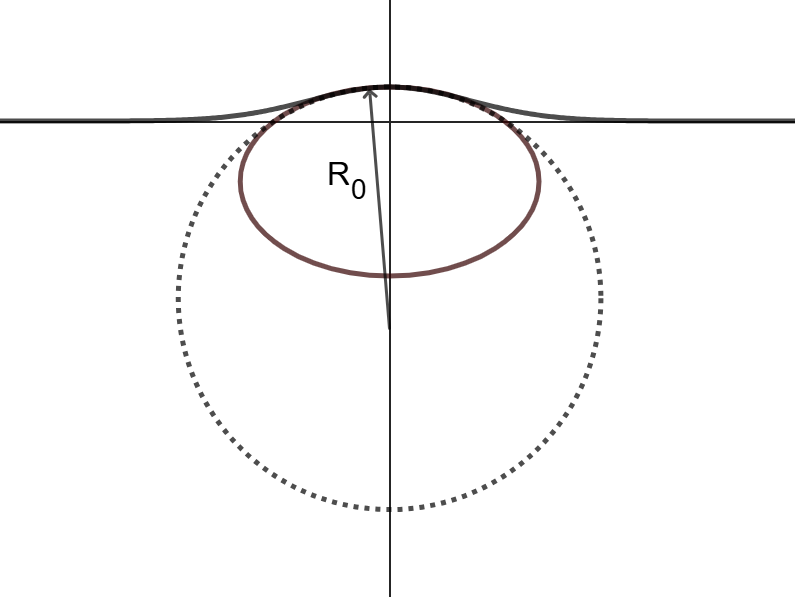
\includegraphics[width=0.55\linewidth]{WriteUp/images/bubble at surface.png}
    \caption{A bubble floating at a surface}
    \label{fig:1}
\end{figure}

We can divide the surface of a bubble into three regions: (A) the submerged portion of the interface, (B) the thin film over the top of the bubble separating the two gas regions, (C) the regions of the interface trailing away from the border of the thin film. We neglect the thickness of the film means we can ignore the weight of the film. Adding that the difference between the gas pressures inside and out of the bubble is uniform, the thin film can be treated as a spherical surface of radius $R_0$. The force balance equations at any point on these surfaces are,
\begin{align}\label{A_untransformed}
    (\rho-\rho')gz = \gamma(\frac{1}{R_1}+\frac{1}{R_2}-\frac{4}{R_0})
\end{align}
for region (A),
\begin{align}\label{B_untransformed}
    p=p_0 + \frac{4\gamma}{R_0}
\end{align}
for region (B),
\begin{align}\label{C_untransformed}
    (\rho-\rho')gz = \gamma(\frac{1}{R_1}+\frac{1}{R_2})
\end{align}
for region (C) where $\gamma$ represents surface tension of the liquid, $g$ is acceleration due to gravity, $\rho$ and $\rho'$ are the densities of the liquid and gas respectively, $p$ and $p_0$ are the gas pressure inside and outside the bubble respectively, $g$ is acceleration due to gravity and $z$ is the height above the still gas liquid interface in the far field. $R_1$ and $R_2$ are the principle radii of curvature of the surface at a point.

In order to calculate what $R_1$ and $R_2$ are we need to use some differential geometry. We assume the bubble can be described by a surfaces of revolution.
Let $\Gamma$ be a curve that lies in the plane $(x,z)$ and let its equation have the equation $z=f(x)$. We then denote $\Phi$ as the surface defined by a rotation of $\Gamma$ around the $z$-axis or axis of rotation. This surface can then be written in the form:
\begin{align}
    z=f(\sqrt{x^2+y^2})=f(r) && r=\sqrt{x^2+y^2}
\end{align}

Then using the formulas derived in \cite{toponogov2006differential} we get
\begin{align}
    E&=1+(\frac{x}{r}f')^2,&G&=1+(\frac{y}{r}f')^2, &F&=\frac{xy}{r^2}(f')^2, &EG-F^2=&1+(f')^2,
\end{align}
for the coefficients of the first fundamental form given by
\begin{align}
    I( \vec{ \boldsymbol\lambda}) = E(\lambda_1)^2 +2F\lambda_1 \lambda_2 + G(\lambda_2)^2
\end{align}
where $\lambda$ is some tangent vector. We can exploit the fact that since our surface is radially symmetric, we only need to find these geometric characteristics on some meridian of the surface, say y=0:
\begin{align}
    E&=1+(f')^2,& G&=1, &F&=0.
\end{align}
Again using the formulas in \cite{toponogov2006differential}, we obtain
\begin{align}
    L&=\frac{f''}{\sqrt{1+(f')^2}},&M&=0&  N&=\frac{f'}{x\sqrt{1+(f')^2}}
\end{align}
for the coefficients of the second fundamental form given by
\begin{align}
    II( \vec{ \boldsymbol\lambda},\vec{ \boldsymbol\mu}) = L\lambda_1 \mu_1 +M(\lambda_1\mu_2 + \lambda_2 \mu_1)  + N\lambda_2 \mu_2.
\end{align}
We then obtain the principle curvatures $\kappa_1$ and $\kappa_2$ satisfy:
\begin{align}
    (EG-F^2)\kappa^2 - (EN+GL -2MF)\kappa +LN-M^2 = 0.
\end{align}
Substituting in our coefficients for the first and second fundamental forms, solving for $\kappa$ and noting radius of curvature is one over the curvature we obtain:
\begin{align}
    \frac{1}{R_1} =\kappa_1= \frac{L}{E}=\frac{f''}{(1+(f')^2)^{\frac{3}{2}}}, && \frac{1}{R_2} = \kappa_2 = \frac{N}{G} = \frac{f'}{x \sqrt{1+(f')^2}}
\end{align}
Notice that $R_1$ is exactly the radius of curvature of the meridian curve $\Gamma$
We now introduce the variable $\phi$ defined to be the angle at which the tangent to $\Gamma$ makes with the x-axis. 
\begin{figure}[hb]
    \centering
    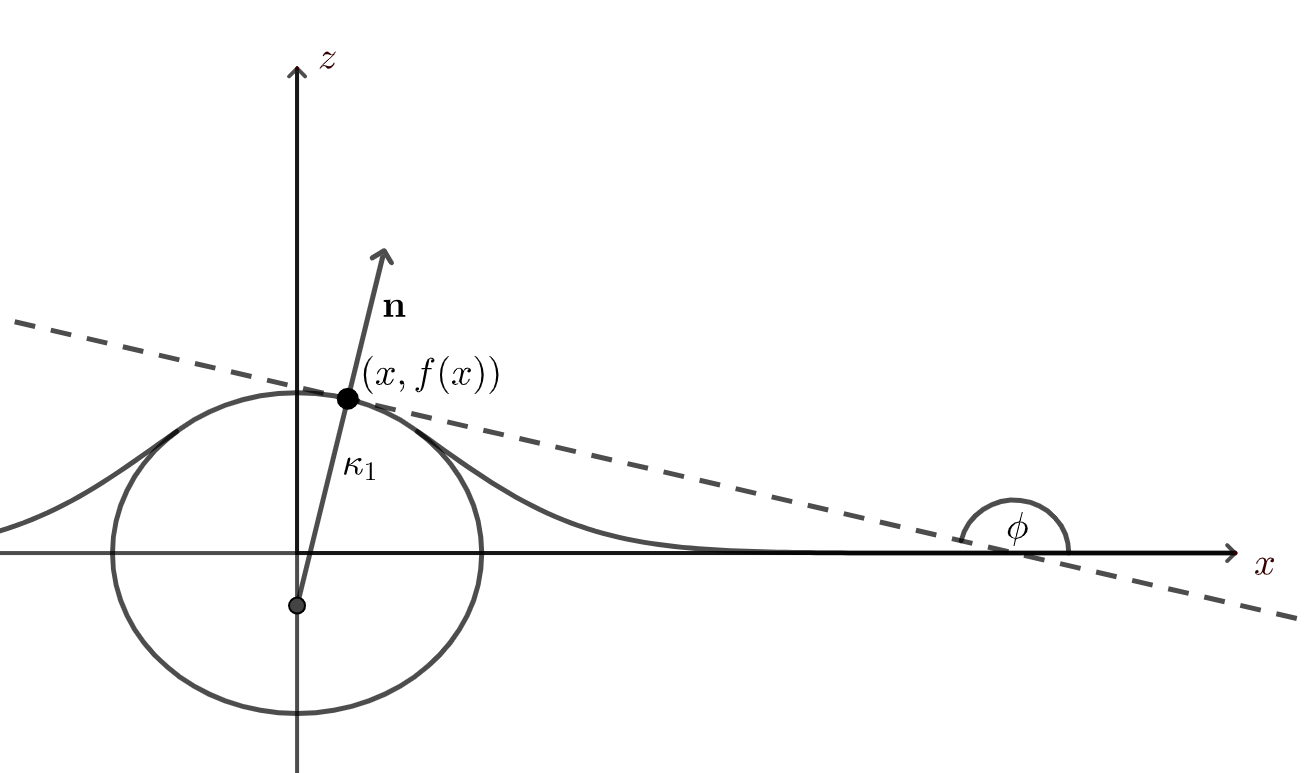
\includegraphics[width=0.55\linewidth]{WriteUp/images/tangent to bubble extra.png}
    \caption{A bubble floating at a surface}
    \label{fig:1}
\end{figure}
We can calculate $\phi$ using simple trigonometry to be $\phi=\arctan(f'(x))$. We then consider:
\begin{align}
    f'(x)=\tan \phi &= \frac{\sin\phi}{\cos\phi} \\
    &=\sin\phi\sec\phi \\
    &=\sin\phi \sqrt{1+\tan^2\phi}\\
    \frac{f'(x)}{\sqrt{1+f'(x)^2}}&=\sin\phi\\
    \frac{d}{dx} \frac{f'(x)}{\sqrt{1+f'(x)^2}}&=\frac{d}{dx}\sin\phi \\
    \frac{f''(x)}{(1+f'(x)^2)^{\frac{3}{2}}}&=\frac{d(\sin\phi)}{dx} \\
    \frac{1}{R_1}&=\frac{d(\sin\phi)}{dx}
\end{align}
Allowing us to obtain $R_1$ in terms of $\phi$. reparametrising the curve in terms of $z$, i.e. considering the curve given by $(g(z),z)$ where $g(z)=f^{-1}(z)$, we can find another expression for $R_1$. using the facts,
\begin{align}
    f'(x)=\frac{1}{g'(f(x))}, && f''(x) = \frac{-g''(f(x))}{g'(f(x))^3}
\end{align}
We can write the curvature in terms of $z$:
\begin{align}
    \frac{f''(x)}{(1+f'(x)^2)^{\frac{3}{2}}}=\frac{-\frac{g''(f(x))}{g'(f(x))^3}}{(1+\frac{1}{g'(f(x))})} = \frac{-g''(f(x))}{(g'(f(x))^2+1)^{\frac{3}{2}}} = \frac{-g''(z)}{(g'(z)+1)^{\frac{3}{2}}}
\end{align}
Now we can consider,
\begin{align}
    f'(x)=\frac{1}{g'(f(x))}=\tan \phi &= \frac{\sin\phi}{\cos\phi} \\
    g'(z)&=\cos\phi\csc\phi \\
    &=\sin\phi \sqrt{1+\cot^2\phi}\\
    \frac{g'(z)}{\sqrt{1+g'(z)^2}}&=\cos\phi\\
    \frac{d}{dz} \frac{f'(z)}{\sqrt{1+f'(z)^2}}&=\frac{d}{dz}\cos\phi \\
    \frac{g''(z)}{(1+g'(z)^2)^{\frac{3}{2}}}&=\frac{d(\cos\phi)}{dx} \\
    \frac{1}{R_1}&=-\frac{d(\cos\phi)}{dz}
\end{align}
We can also write $R_2$ in terms of $\phi$ by considering the normal to the curve at a point $(x,f(x))$. An equation for this normal is given by
\begin{align}
    (\bar{x}-x) + f'(x)(\bar{z}-f(x))=0
\end{align}
where $(\bar{x},\bar{z})$ are the coordinates of points on the straight line. We can the find the intersection of this line with the $z$-axis, $(0,\frac{x+ff'}{f'})$.
Finding the distance $R$ between this point and $(x,f)$ gives
\begin{align}
    R=\sqrt{x^2+(\frac{x+ff'}{f'}-f)^2}=\frac{x\sqrt{1+(f')^2}}{|f'|}=R_2.
\end{align}
We can then use trigonometry to calculate $R$ in terms of $\phi$:
\begin{align}
    R=\frac{x}{\cos(\frac{\pi}{2}-\phi)}=\frac{x}{\sin(\phi)}.
\end{align}
Combining these all together we obtain
\begin{align}
    \frac{1}{R_1}&=\frac{d(\sin(\phi))}{dx},\\
    \frac{1}{R_2}&=\frac{\sin(\phi)}{x},\\
    \frac{dz}{dx} &= \tan(\phi).
\end{align}
\begin{figure}[hb]
    \centering
    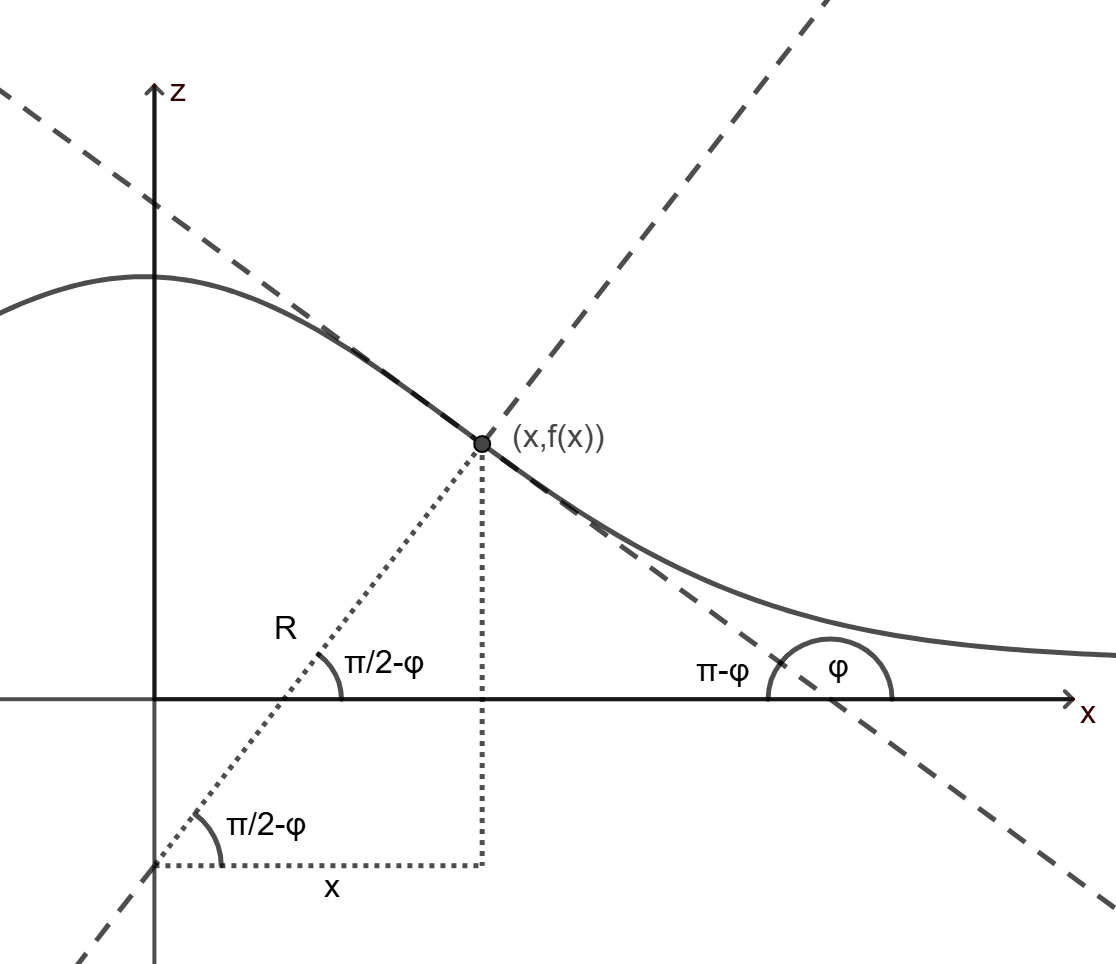
\includegraphics[width=0.6\linewidth]{WriteUp/images/angles and trig.png}
    \caption{A bubble floating at a surface}
    \label{fig:4}
\end{figure}
We now introduce a capillary constant $a^2$ having dimension of square length and defined by the equation
\begin{align}
    \frac{(\rho-\rho')g}{\gamma} = \frac{2}{a^2}
\end{align}
transform $x$, $z$, $R_0$, etc. to dimensionless quantities $\bar{x}$, $\bar{z}$, $\bar{R_0}$, etc. by
\begin{align}
    x=a\bar{x}, && z=a\bar{z}, && R_0=a\bar{R}_0, && \text{etc.}
\end{align}
We then consider two new transformed coordinates:
\begin{align}
    \bar{z}_1 = \bar{z}+\bar{h}, && \bar{z}_2=\bar{z}+\bar{l}
\end{align}
where $\bar{h}$ and $\bar{l}$ are chosen such that $\bar{z}_1$ has its origin at the deepest point of the bubble for portion (A) and $\bar{z}_2$ has its origin at the centre of the sphere for portion (B). For portion (A), instead of \ref{A_untransformed}, we obtain
\begin{align}\label{less than}
\begin{rcases}   
    \frac{d\bar{z}_1}{d\bar{x}} &= \tan \phi \\
    \frac{d(\sin\phi)}{d\bar{x}} &= 2\bar{z}_1 - \frac{\sin\phi}{\bar{x}} + \theta
\end{rcases} 
\end{align}
or,
\begin{align}\label{greater than}
\begin{rcases}
    \frac{d\bar{x}}{d\bar{z}_1} &= \cot \phi \\
    \frac{d(\cos\phi)}{d\bar{z}_1} &= -2\bar{z}_1 + \frac{\sin\phi}{\bar{x}} - \theta
\end{rcases}
\end{align}
where,
\begin{align}
    \theta = \frac{4}{\bar{R}_0} - 2\bar{h}
\end{align}
and the equations \ref{less than} and \ref{greater than} are used for $\tan\phi <1$ and $\tan\phi >1$ respectively. Similarly for portion (C), equation \ref{C_untransformed} becomes,
\begin{align}\label{C_transformed}
\begin{rcases}   
    \frac{d\bar{z}}{d\bar{x}} &= \tan \phi \\
    \frac{d(\sin\phi)}{d\bar{x}} &= 2\bar{z} - \frac{\sin\phi}{\bar{x}}
\end{rcases} 
\end{align}
We can notice that equation \ref{less than} and \ref{greater than} are essentially the same of equation \ref{C_transformed} except for the additional $\theta$ term. Finally equation \ref{B_untransformed} for portion (B) becomes
\begin{align}\label{Eq_B}
    \bar{z}_2 = \sqrt{ \bar{R}_0^2+\bar{x}^2}
\end{align}
We are now ready to start solving for the initial condition.

\subsection{Solving Portion (A)}

We have derived the governing equations for each of the three portions of the bubble and now can start to solve them. We already have an explicit expression for portion (B), although finding analytic solutions to \ref{less than}, \ref{greater than} and \ref{C_transformed} is too difficult. Instead we can find numerical solutions using a Runge-Kutta method.

First we consider the equations \ref{less than} and \ref{greater than}. We use the initial conditions $\bar{x}=\bar{z}_1=0$ at $\theta=0$ as we assume that at the bottom of the bubble is flat, i.e.
\begin{align}
    \frac{d\bar{z}_1}{d\bar{x}}&=0\\
    \Leftrightarrow \:\:\:\:\:\theta&=0.
\end{align}
The relations
\begin{align}
    \frac{1}{\bar{R}_1}=\frac{\sin\phi}{\bar{x}}=\frac{1}{\bar{R}_2}=\frac{d(\sin\phi)}{d\bar{x}}=\frac{\theta}{2}
\end{align}
In order to solve this ODE, we used the $\texttt{solve\_ivp}$ function from SciPy \cite{2020SciPy-NMeth}. Once again we need to do a little more work before we're able to use this function. First, consider the vector $\bf{z}$ defined by
\begin{align}
    \bf{z} = \begin{bmatrix}
           \bar{z}_1 \\
           u \\
         \end{bmatrix}
\end{align}
where $u=\sin \phi$. Transforming our ODE we obtain
\begin{align}
    \frac{d\bf{z}}{d\bar{x}}=\begin{bmatrix}
           \frac{u}{\sqrt{1-u^2}} \\
           -2\bar{z}_1 - \frac{u}{\bar{x}}+\theta \\
         \end{bmatrix}
\end{align}
which we can then solve for $\phi \in [0,\pi]$.
\begin{figure}[hb]
    \centering
    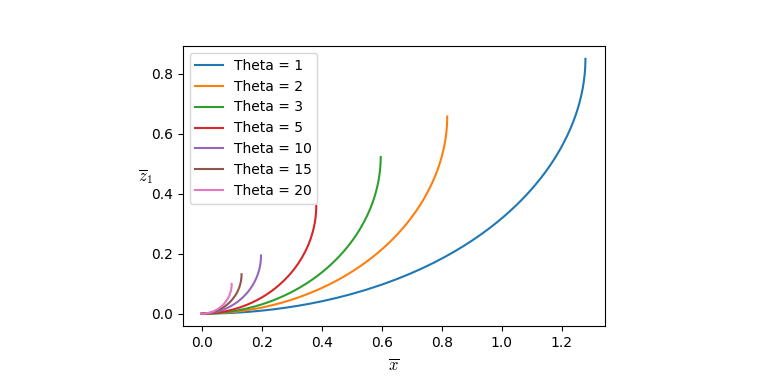
\includegraphics[width=0.85\linewidth]{WriteUp/images/bottom curve.png}
    \caption{Solutions to \ref{less than} for various $\theta$ values}
    \label{fig:9}
\end{figure}
As $\phi \rightarrow \pi/2$, $\frac{d\bar{z}_1}{dx} \rightarrow \infty$. This means our solver cannot compute the solution for $\phi> \pi/2$. What we do instead, is we can use the computed values for $\bar{z}_1$ and $\bar{x}$ at $\phi=\pi/2$ as initial conditions for equations \ref{greater than}. In a similar way to before, we can transform the equations \ref{greater than} into
\begin{align}
     \frac{d\bf{x}}{d\bar{z}_1}=\begin{bmatrix}
           \frac{v}{\sqrt{1-v^2}} \\
           -2\bar{z}_1 + \frac{\sqrt{1-v^2}}{\bar{x}}-\theta \\
         \end{bmatrix},
\end{align}
where $ \bf{x} = \begin{bmatrix}
    \bar{x}\\v
\end{bmatrix}$ and $v=\cos\phi$. We can then once again use $\texttt{solve\_ivp}$ to get a full solution to \ref{less than} and \ref{greater than}.let this solution be denoted by the function $F$ where
\begin{align}
    F(\bar{x},\theta,\phi)= \begin{cases}
        f_1(\bar{x},\theta) \;\;\;\;\; \text{for } \phi>\pi/2\\
        \tilde{f_1}(\bar{x},\theta) \;\;\;\;\; \text{for } \phi<\pi/2
    \end{cases}
\end{align}

\begin{figure}[hb]
    \centering
    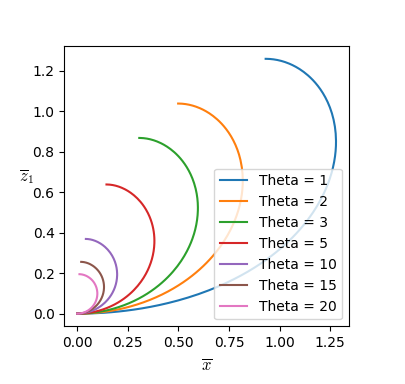
\includegraphics[width=0.85\linewidth]{WriteUp/images/top and bottom curve.png}
    \caption{Solutions to \ref{less than} and \ref{greater than} for various $\theta$ values}
    \label{fig:10}
\end{figure}

\subsection{Solving Portion (C)}

The equations generating portion (C) are very similar to portion (A), unfortunately, the boundary conditions make it much harder to solve. Portion (C) is the meniscus of the bubble and we would like it to flatten out at infinity. This means we have the boundary conditions $\phi \rightarrow 0$, $\bar{z} \rightarrow 0$ as $x \rightarrow \infty$. These conditions are unable to be implemented numerically, instead we can consider initial conditions close to zero, i.e. $\bar{z}=\phi=0.00001$ at $\bar{x}=\bar{x}_0$. We can then denote $\bar{z}=f_2(\bar{x},\bar{x}_0)$ as a solution to \ref{C_transformed}

\begin{figure}[hb]
    \centering
    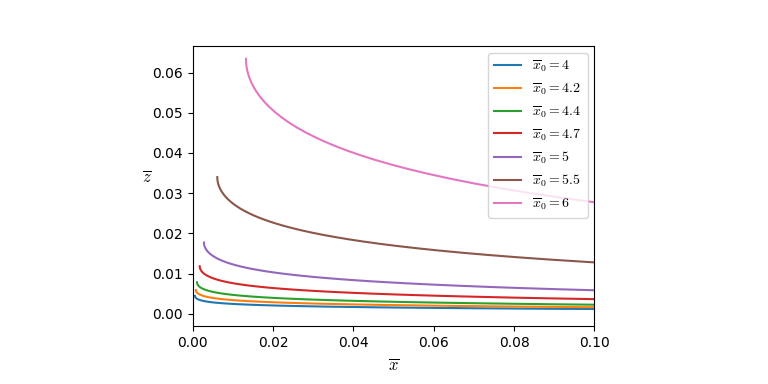
\includegraphics[width=0.85\linewidth]{WriteUp/images/menisc.png}
    \caption{Solutions to \ref{C_transformed} for various $\bar{x}_0$ values}
    \label{fig:10}
\end{figure}

\subsection{Combining all the portions}

We are now able to calculate an explicit description of the interface for each individual section, but we still have many unknown variables we need to solve for. We want each portion to meet at the same point and match derivatives at that point. applying these constraints we get the following system of equations:
\begin{align}
    \bar{z}&=F(\bar{x},\theta,\phi) - \bar{h} \\
    \bar{z}&=f_2(\bar{x},\bar{x}_0) \\
    \bar{z}&=\sqrt{\bar{R}_0^2-\bar{x}^2} - \bar{l}=f_3(\bar{x},\bar{R}_0)-\bar{l} \\
    \theta&=\frac{4}{\bar{R}}-2\bar{h}
\end{align}
and
\begin{align}
    \frac{d}{d\bar{x}}F(\bar{x},\theta,\phi)&=\frac{d}{d\bar{x}}f_2(\bar{x},\bar{x}_0) = \frac{d}{d\bar{x}}f_3(\bar{x},\bar{R}_0)
\end{align}
We can notice that $\frac{d}{d\bar{x}}f_3(\bar{x},\bar{R}_0)$ is always negative and that $\frac{d}{d\bar{x}}F(\bar{x},\theta,\phi)$ is only negative when $\phi>\pi/2$, i.e. when $F(\bar{x},\theta,\phi)=f_1(\bar{x},\theta)$. Using this we can reduce our system down to seven unknowns and six equations to solve.
In order to solve this, we can
\section{Conclusion}

In summary, this has been a very successful project.


\pagebreak

{\Huge \bf Bibliography}

\bigskip

% These are examples of the book titles as they can be put in. 
% You can use different labeling methods, if you prefer, 
% e.g., just enumerating the items  as [1], [2], etc.,
% instead of making them [ATLAS], [B], etc.
% Or use bibtex

\bibliographystyle{unsrtnat}
\bibliography{WriteUp/refs}


\end{document}
